\documentclass[titlepage, a4paper]{article}
\usepackage[swedish]{babel}
\usepackage[utf8]{inputenc}
\usepackage{color}

% Sidformat
\usepackage{a4wide}

% Fixa Appendix-titlar
\usepackage[titletoc,title]{appendix}

% Bättre bildtexter
\usepackage[margin=10pt,font=small,labelfont=bf,labelsep=endash]{caption}

% Enkelt kommando som låter mig attgöra-markera text
\newcommand{\todo}[1] {\textbf{\textcolor{red}{#1}}}

%% Headers och Footers
\usepackage{fancyhdr}
\pagestyle{fancy}
\lhead{}
\rhead{\today}
\lfoot{\LIPSkursnamn \\ \LIPSdokumenttyp}
\cfoot{\thepage}
\rfoot{\LIPSprojektgrupp \\ \LIPSprojektnamn}

%% Titelsida
\newcommand{\LIPSTitelsida}{%
{\ }\vspace{45mm}
\begin{center}
  \textbf{\Huge \LIPSdokument}
\end{center}
\begin{center}
  {\Large Redaktör: \LIPSredaktor}
\end{center}
\begin{center}
  {\Large \textbf{Version \LIPSversion}}
\end{center}
\vfill
\begin{center}
  {\large Status}\\[1.5ex]
  \begin{tabular}{|*{3}{p{40mm}|}}
    \hline
    Granskad & \LIPSgranskare & \LIPSgranskatdatum \\
    \hline
    Godkänd & \LIPSgodkannare & \LIPSgodkantdatum \\
    \hline
  \end{tabular}
\end{center}
\newpage
}


% Projektidentitet
\newenvironment{LIPSprojektidentitet}{%
{\ }\vspace{45mm}
\begin{center}
  {\Large PROJEKTIDENTITET}\\[0.5ex]
  {\small
  \LIPSartaltermin, \LIPSprojektgrupp\\
  Linköpings Tekniska Högskola, MAI
  }
\end{center}
\begin{center}
  {\normalsize Gruppdeltagare}\\
  \begin{tabular}{|l|l|p{25mm}|l|}
    \hline
    \textbf{Namn} & \textbf{Ansvar} & \textbf{Telefon} & \textbf{E-post} \\
    \hline
}%
{%
    \hline
  \end{tabular}
\end{center}
\begin{center}
  {\small
    \textbf{E-postlista för hela gruppen}: \LIPSgruppadress\\
    \textbf{Hemsida}: \LIPSgrupphemsida\\[1ex]
    \textbf{Kund}: \LIPSkund\\
    \textbf{Kontaktperson hos kund}: \LIPSkundkontakt\\
    \textbf{Kursansvarig}: \LIPSkursansvarig\\
    \textbf{Handledare}: \LIPShandledare\\
  }
\end{center}
\newpage
}
\newcommand{\LIPSgruppmedlem}[4]{\hline {#1} & {#2} & {#3} & {#4} \\}

%% Dokumenthistorik
\newenvironment{LIPSdokumenthistorik}{%
\begin{center}
  Dokumenthistorik\\[1ex]
  %\begin{small}
    \begin{tabular}{|l|l|p{60mm}|l|l|}
      \hline
      \textbf{Version} & \textbf{Datum} & \textbf{Utförda förändringar} & \textbf{Utförda av} & \textbf{Granskad} \\
      }%
    {%
			\hline
    \end{tabular}
  %\end{small}
\end{center}
}

\newcommand{\LIPSversionsinfo}[5]{\hline {#1} & {#2} & {#3} & {#4} & {#5} \\}

% Kravlistor
\newenvironment{LIPSkravlista}{
	\center
		\tabularx{\textwidth}{| p{1.2cm} | p{1.9cm} | X | c |}
			\hline
			\textbf{Krav} & \textbf{Förändring} & \textbf{Beskrivning} & \textbf{Prioritet} \\\hline
}
{
		\endtabularx
	\endcenter
}

\newcounter{LIPSkravnummer}
\addtocounter{LIPSkravnummer}{1}
\newcommand{\LIPSkrav}[4][Krav \arabic{LIPSkravnummer}]{{#1} & {#2} & {#3} & {#4} \stepcounter{LIPSkravnummer}\\\hline}	% Importera generella layout-strukturer

% Information nödvändig för generella layout-strukturer
\newcommand{\LIPSredaktor}{Pål Kastman}
\newcommand{\LIPSversion}{0.1}
\newcommand{\LIPSdokument}{Systemskiss}
\newcommand{\LIPSdokumenttyp}{Systemskiss}
\newcommand{\LIPSgranskatdatum}{}
\newcommand{\LIPSgranskare}{}
\newcommand{\LIPSgodkannare}{}
\newcommand{\LIPSgodkantdatum}{}
\newcommand{\LIPSkursnamn}{TSEA29}
\newcommand{\LIPSprojektnamn}{Lagerrobot}
\newcommand{\LIPSprojektgrupp}{Grupp 2}
%\newcommand{\LIPSgruppadress}{}
\newcommand{\LIPSartaltermin}{HT1, 2014}	
\newcommand{\LIPSgrupphemsida}{http://github.com/ultralaserdeluxe/gloria}
\newcommand{\LIPSkund}{Tomas Svensson}
\newcommand{\LIPSkundkontakt}{Tomas Svensson}
\newcommand{\LIPSkursansvarig}{Tomas Svensson}
\newcommand{\LIPShandledare}{Peter Johansson}

% Dokument-specifika paket
\usepackage{tabularx}
\usepackage{tikz}
\usetikzlibrary{shapes, arrows}

\pagenumbering{roman}

\begin{document}

\LIPSTitelsida

\begin{LIPSprojektidentitet}
\LIPSgruppmedlem{Pål Kastman}{Projektledare}{0703896295}{palka285@student.liu.se}
\LIPSgruppmedlem{Hannes Snögren}{Dokumentansvarig}{0706265064}{hansn314@student.liu.se}
\LIPSgruppmedlem{Alexander Yngve}{Hårdvaruansvarig}{0762749762}{aleyn573@student.liu.se}
\LIPSgruppmedlem{Martin Söderén}{Mjukvaruansvarig}{0708163241}{marso329@student.liu.se}
\LIPSgruppmedlem{Daniel Wassing}{Leveransansvarig}{0767741110}{danwa223@student.liu.se}
\LIPSgruppmedlem{Dennis Ljung}{Testansvarig}{0708568148}{denlj069@student.liu.se}
\end{LIPSprojektidentitet}

\newpage
\tableofcontents	%Innehållsförteckning	
%\listoffigures
%\listoftables

\newpage

\begin{LIPSdokumenthistorik}
\LIPSversionsinfo{0.1}{}{Första utkast}{}{}
\end{LIPSdokumenthistorik}

\newpage
\pagenumbering{arabic}	%Påbörja sidnumrering

% Inledning, översikt osv
\section{Inledning}
Systemet kommer bestå av en robot som i sig består av tre undermoduler. Utöver detta tillkommer mjukvara på roboten och PC som används för manuell styrning och övervakning. Detta är en systemskiss som ska ge en grov översikt hur systemet ska implementeras. Detta ska sedan vara underlag för designspecifikationen. 
\newline
\newline
Varje enskild modul kommer att ha en egen processor och dessa kommer sedan kommunicera med varandra. Systemet kommer kommunicera med en PC över blåtand. När systemet är klart för leverans ska det kunna följa en bana som visas nedan och plocka upp och sätta ned paket på de utsatta stationerna B och C. Den ska även kunna detektera avbrott (A) samt slutstation (D). 

\centerline{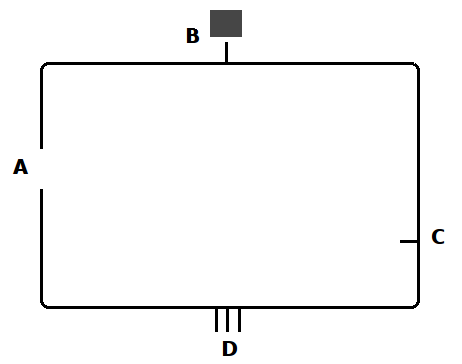
\includegraphics[scale=0.4]{figur}}
\centerline{Banöversikt}
\centerline{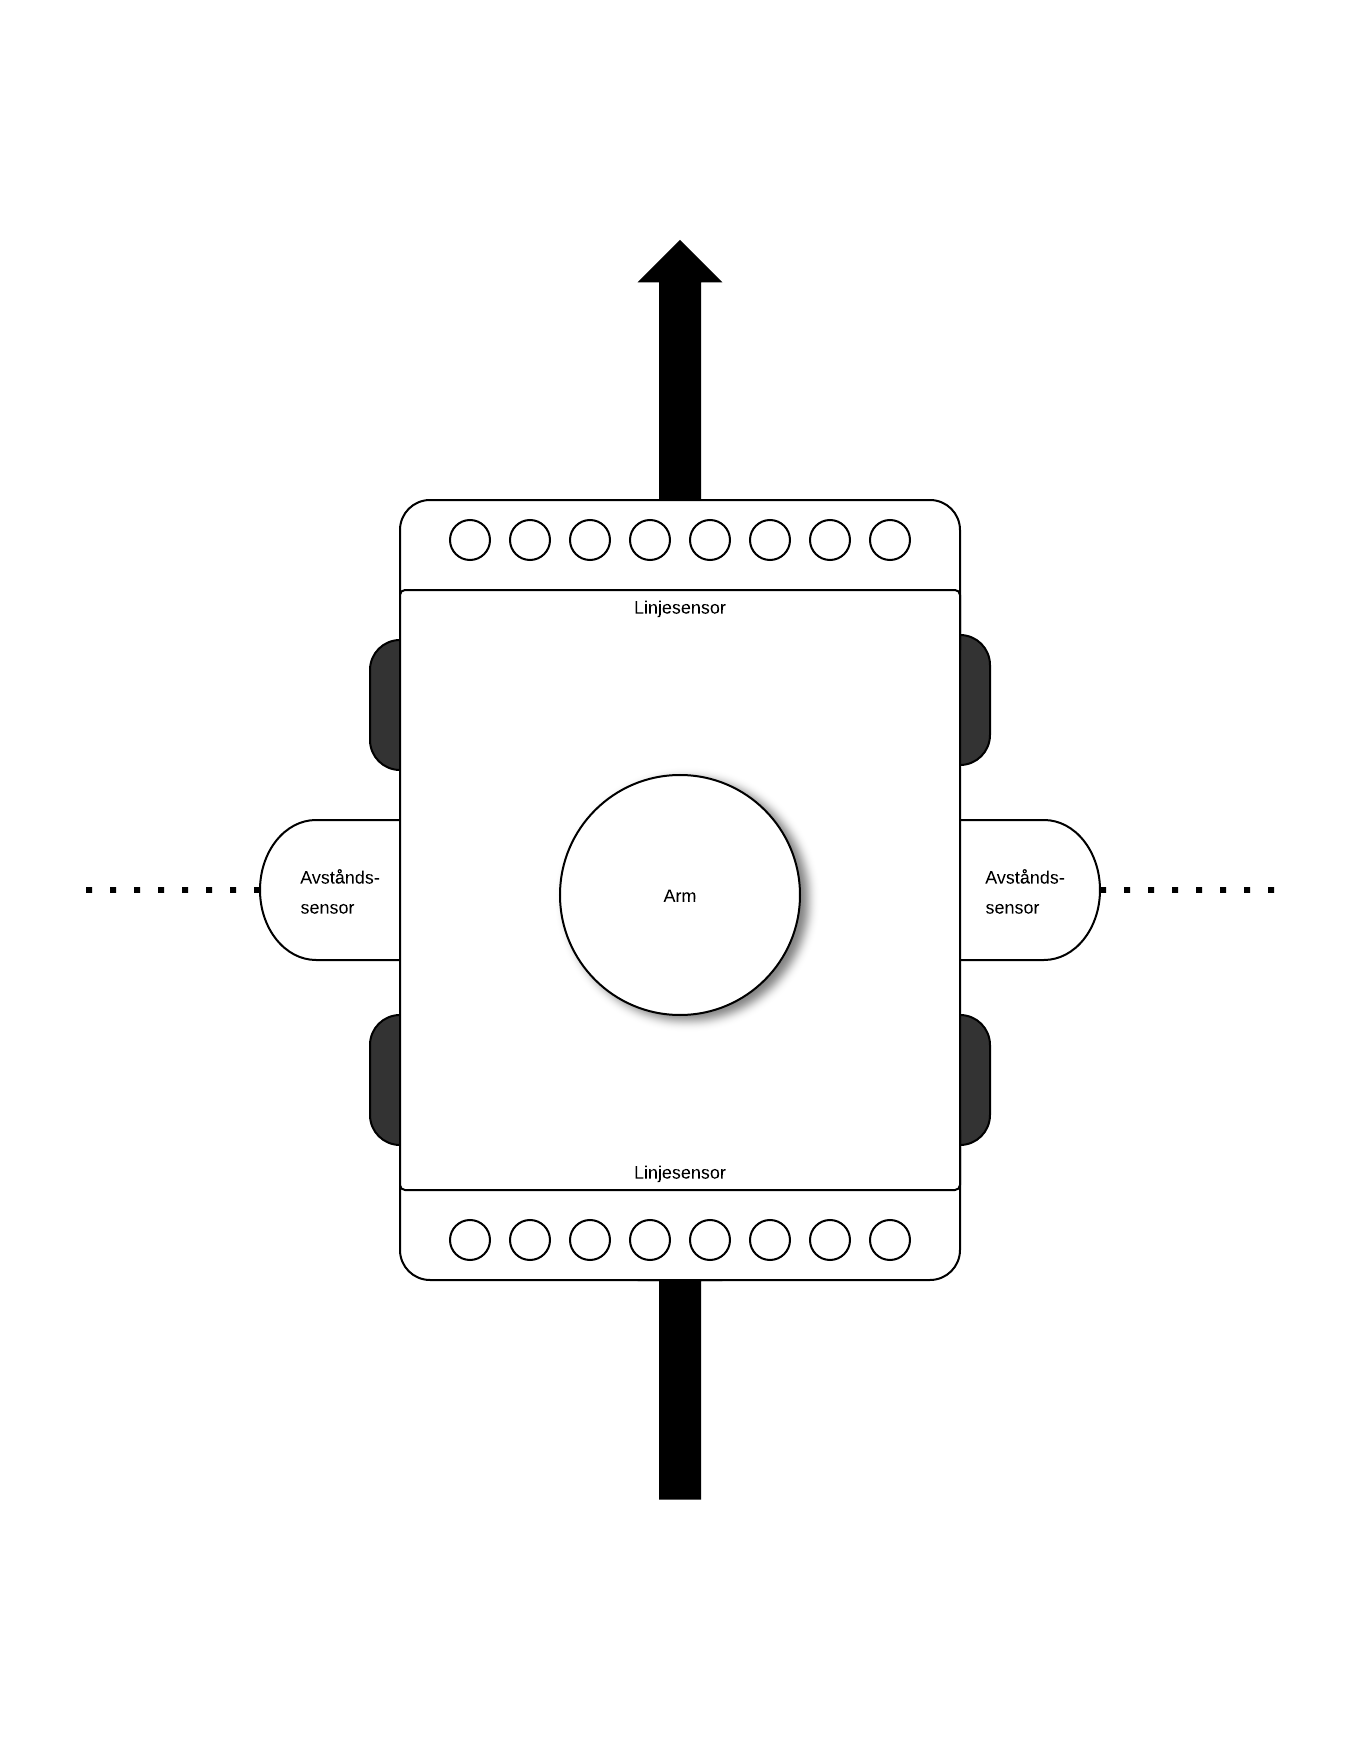
\includegraphics[scale=0.19]{robot}}
\centerline{Robot sedd ovanifrån}	

\section{Översikt av system}
På plattformen kommer tre moduler att installeras:

\begin{itemize}
\item Huvudmodul
\item Styrmodul
\item Sensormodul
\end{itemize}
Huvudmodulen kommer troligvis bestå av en Beagleboard-xM. Sensormodulen och styrmodulen ska förslagsvis bestå av varsin Atmega16.
\subsection{Kommunikation}
Kommunikationen mellan Huvudmodulen, styrmodulen och sensormodulen kommer förslagsvis att ske över UART. Huvudmodulen kommer isåfall ha två stycken USB-RS232 konverterare som kommer kopplas till varsin modul. Kommunikationen från huvudmodulen till PC kommer att ske över Bluetooth. Förslaget är att sätta upp ett PAN (PERSONAL AREA NETWORK) mellan PC:n och huvudmodulen. Detta möjliggör kommunikation över TCP/IP protokollet.
%\newline
%\centerline{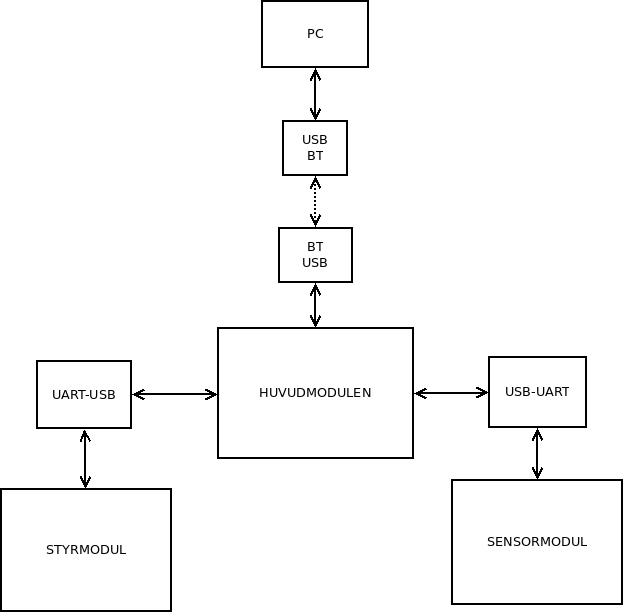
\includegraphics[scale=0.4]{FLOW1PNG}}
%\centerline{Flödesschema över kommunikationen i systemet}
%\newline
%\newline
%\centerline{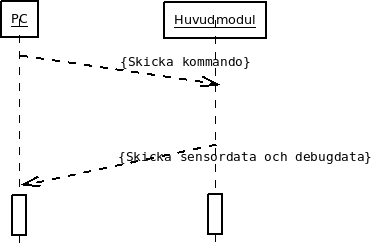
\includegraphics[scale=0.6]{PC-huvud}}
%\centerline{Kommunikation mellan PC och huvudmodulen}
%\newline
%\newline
%\centerline{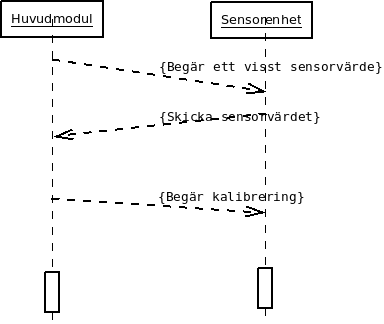
\includegraphics[scale=0.6]{huvud-sensor}}
%\centerline{Kommunikation mellan huvudmodulen och sensormodulen}
%\newline
%\newline
%\centerline{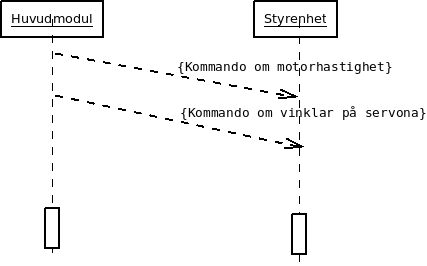
\includegraphics[scale=0.6]{huvud-styr}}
%\centerline{Kommunikation mellan huvudmodulen och styrmodulen}

\begin{figure}[h]
\center
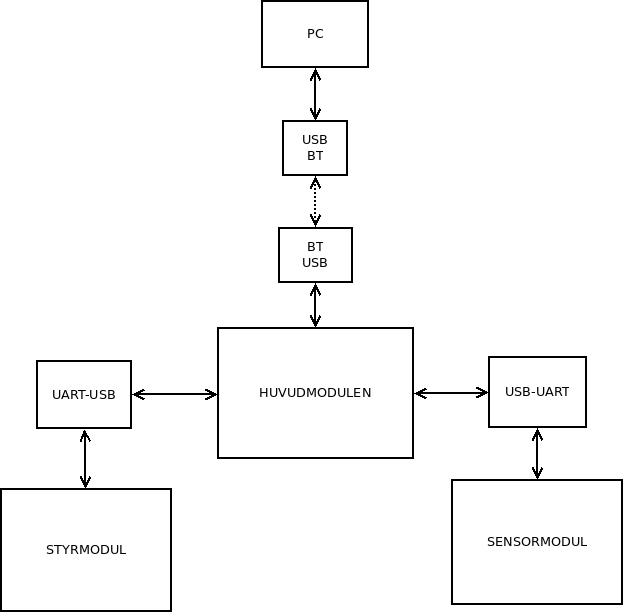
\includegraphics[scale=0.3]{grafik/oversikt-kommunikation}
\caption{Flödesschema över kommunikation i systemet.}
\end{figure}

\begin{figure}[h]
\center
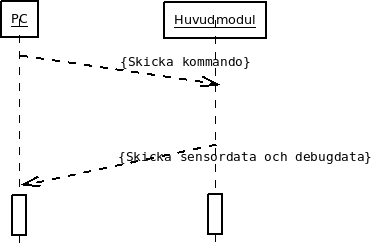
\includegraphics[scale=0.6]{grafik/oversikt-kommunikation-PC-huvud}
\caption{Kommunikation mellan PC och huvudmodulen.}
\end{figure}

\begin{figure}[h]
\center
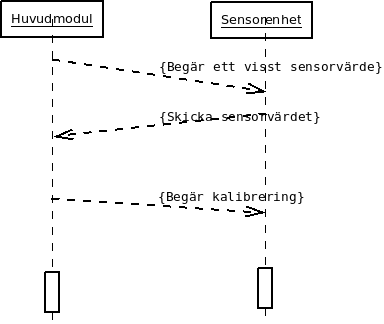
\includegraphics[scale=0.6]{grafik/oversikt-kommunikation-huvud-sensor}
\caption{Kommunikation mellan huvudmodulen och sensormodulen.}
\end{figure}

\begin{figure}[h]
\center
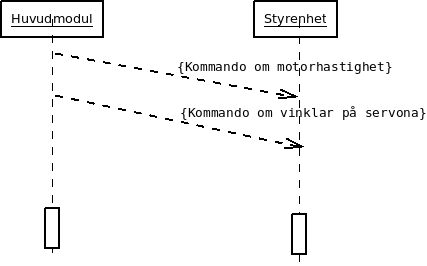
\includegraphics[scale=0.6]{grafik/oversikt-kommunikation-huvud-styr}
\caption{Kommunikation mellan huvudmodulen och styrmodulen.}
\end{figure}

\subsection{Uppgraderbarhet}
Tydliga kommunikationsprotokoll ska existera eftersom det blir enklare att byta ut en modul. Kommunikationen mellan huvudmodulen och övriga moduler sker förslagsvis över UART. Eftersom detta sker med hjälp av USB-UART donglar så finns det möjlighet att lägga till fler moduler i framtiden eftersom Beagleboarden har fyra USB-portar och tre kommer användas i systemet. Behövs fler i framtiden så kan en USB-hubb användas.
\newline
\newline
Kommunikationen mellan huvudmodulen och PC:n kommer förslagsvis att ske över bluetooth och isåfall kommer den användas för att sätta upp ett PAN. Över denna sätts en TCP/IP anslutning upp och data skickas över en Python-socket vilket leder till att bluetooth kan bytas ut mot WIFI eller en ethernetkabel.


\section{Huvudmodul}
Huvudmodulen kan ses som systemets "hjärna". Här sker alla beräkningar för att roboten ska kunna utföra sina uppgifter. Dessa uppgifter ska huvudmodulen hantera antingen via kommandon från en PC eller skötas helt autonomt. Detta är en kritisk modul då den kommer att utföra mycket uppgifter. Den behöver inte mycket hårdvara men den kommer vara mjukvarutung.
\subsection{Hårdvara}
Modulen ska förslagsvis bestå av en enkortsdator av modell Beagleboard. Den har en ARM Cortex-A8 processor som har en klockfrekvens på 1GHz. Denna behöver ett operativsystem för att kunna användas. Den enda hårdvaran som behövs för att kunna använda BB är ett minneskort för operativsystem och en bluetooth-dongel för kommunikationen med PC:n. Även två USB-UART konverterare behövs för kommunikationen med de övriga modulerna.
\subsection{Autonomt läge}
När roboten är satt i autonomt läge kommer all styrning skötas av en algoritm i huvudmodulen, med undantag för upphämtning av paket där användaren styr armen. Detta är en väldigt kritisk del då detta är denna algoritm som avgör robotens beteende och som sedan kommer leda till att den kan fullfölja sina uppgifter. Troligtvis kommer en stor del av tiden läggas på att felsöka och optimera algoritmen.
För att roboten ska kunna färdas framåt smidigt så kommer den behöva någon slags reglering. Förslagsvis ska en PD reglering implementeras som arbetar tidsdiskret. Detta gör att man måste sampla data från linjesensorerna med att visst intervall. Detta intervall är ej bestämt än.
%\newline
%\newline
%\centerline{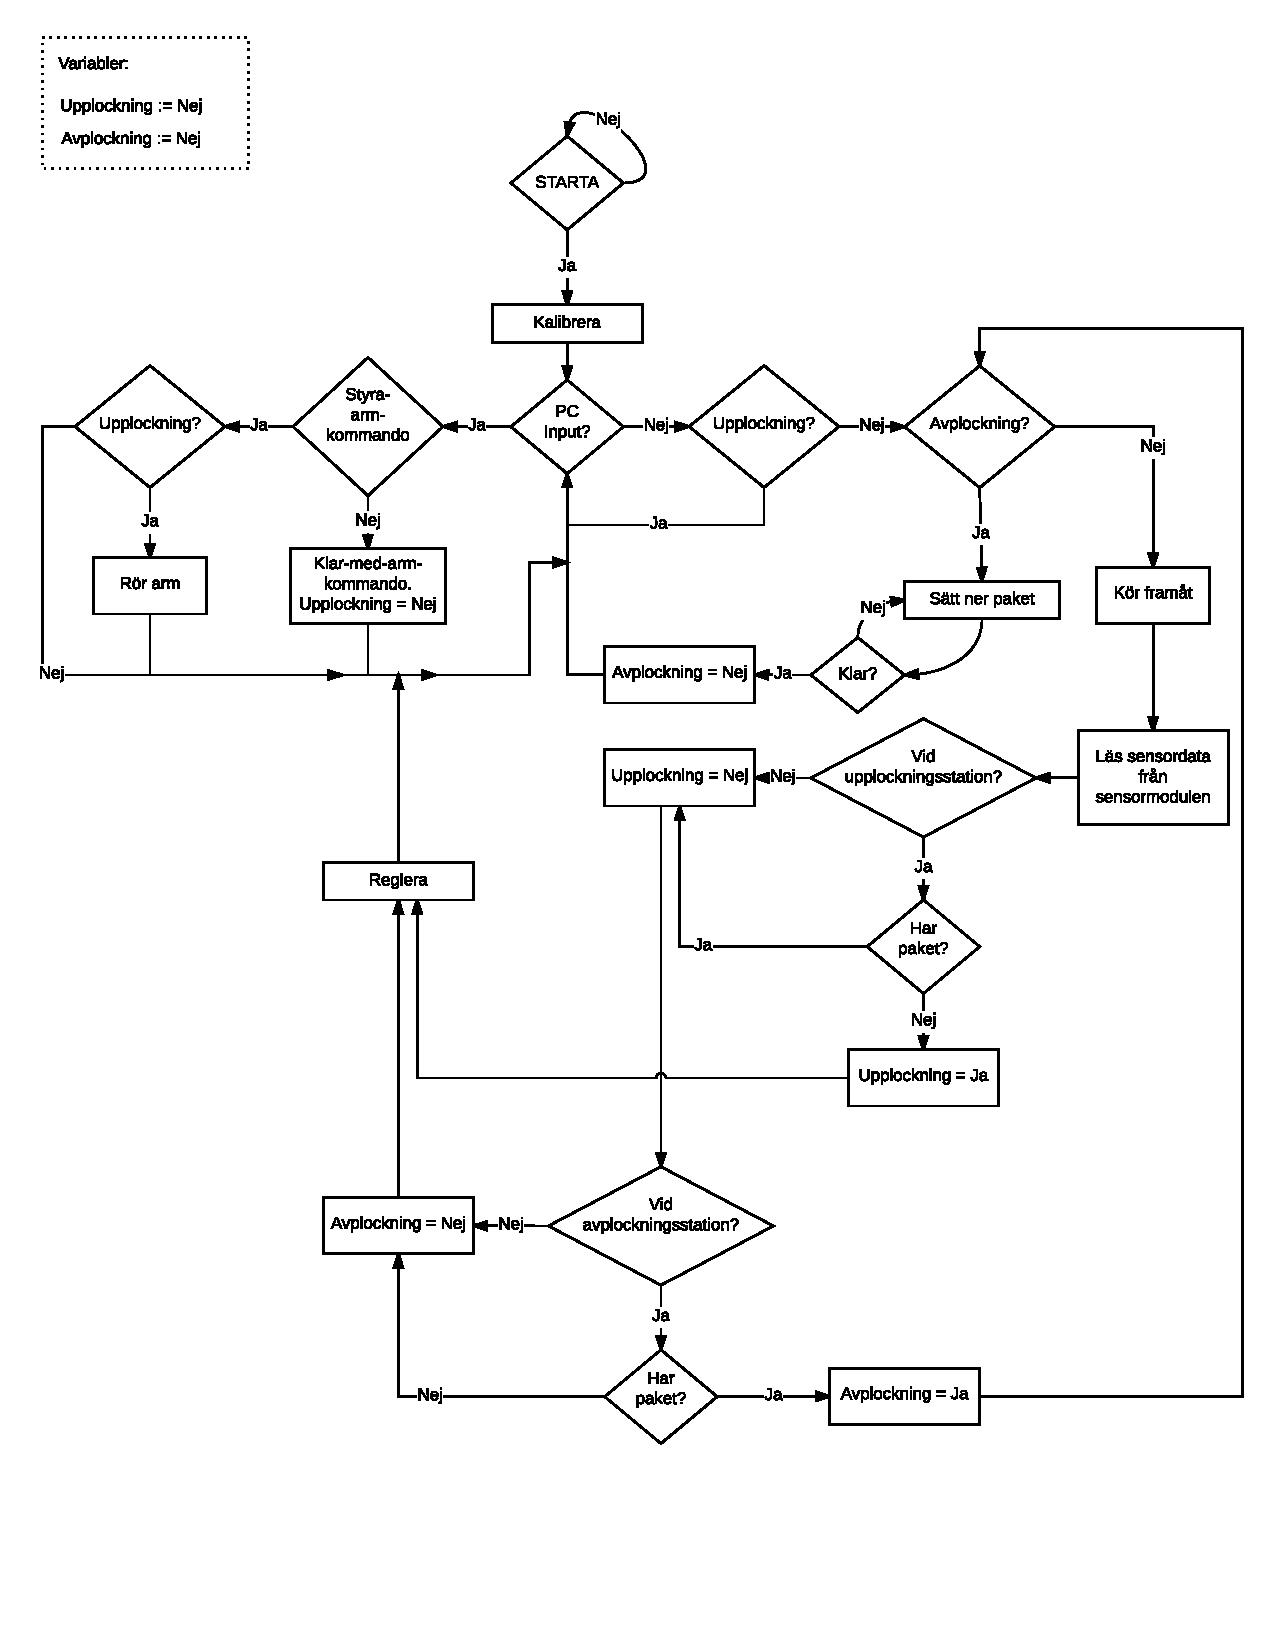
\includegraphics[scale=0.6]{Styrlogik.pdf}}
%\centerline{Flödesschema för huvudmodules styralgoritm}
%\newline
%\newline


\begin{figure}[h]
\center
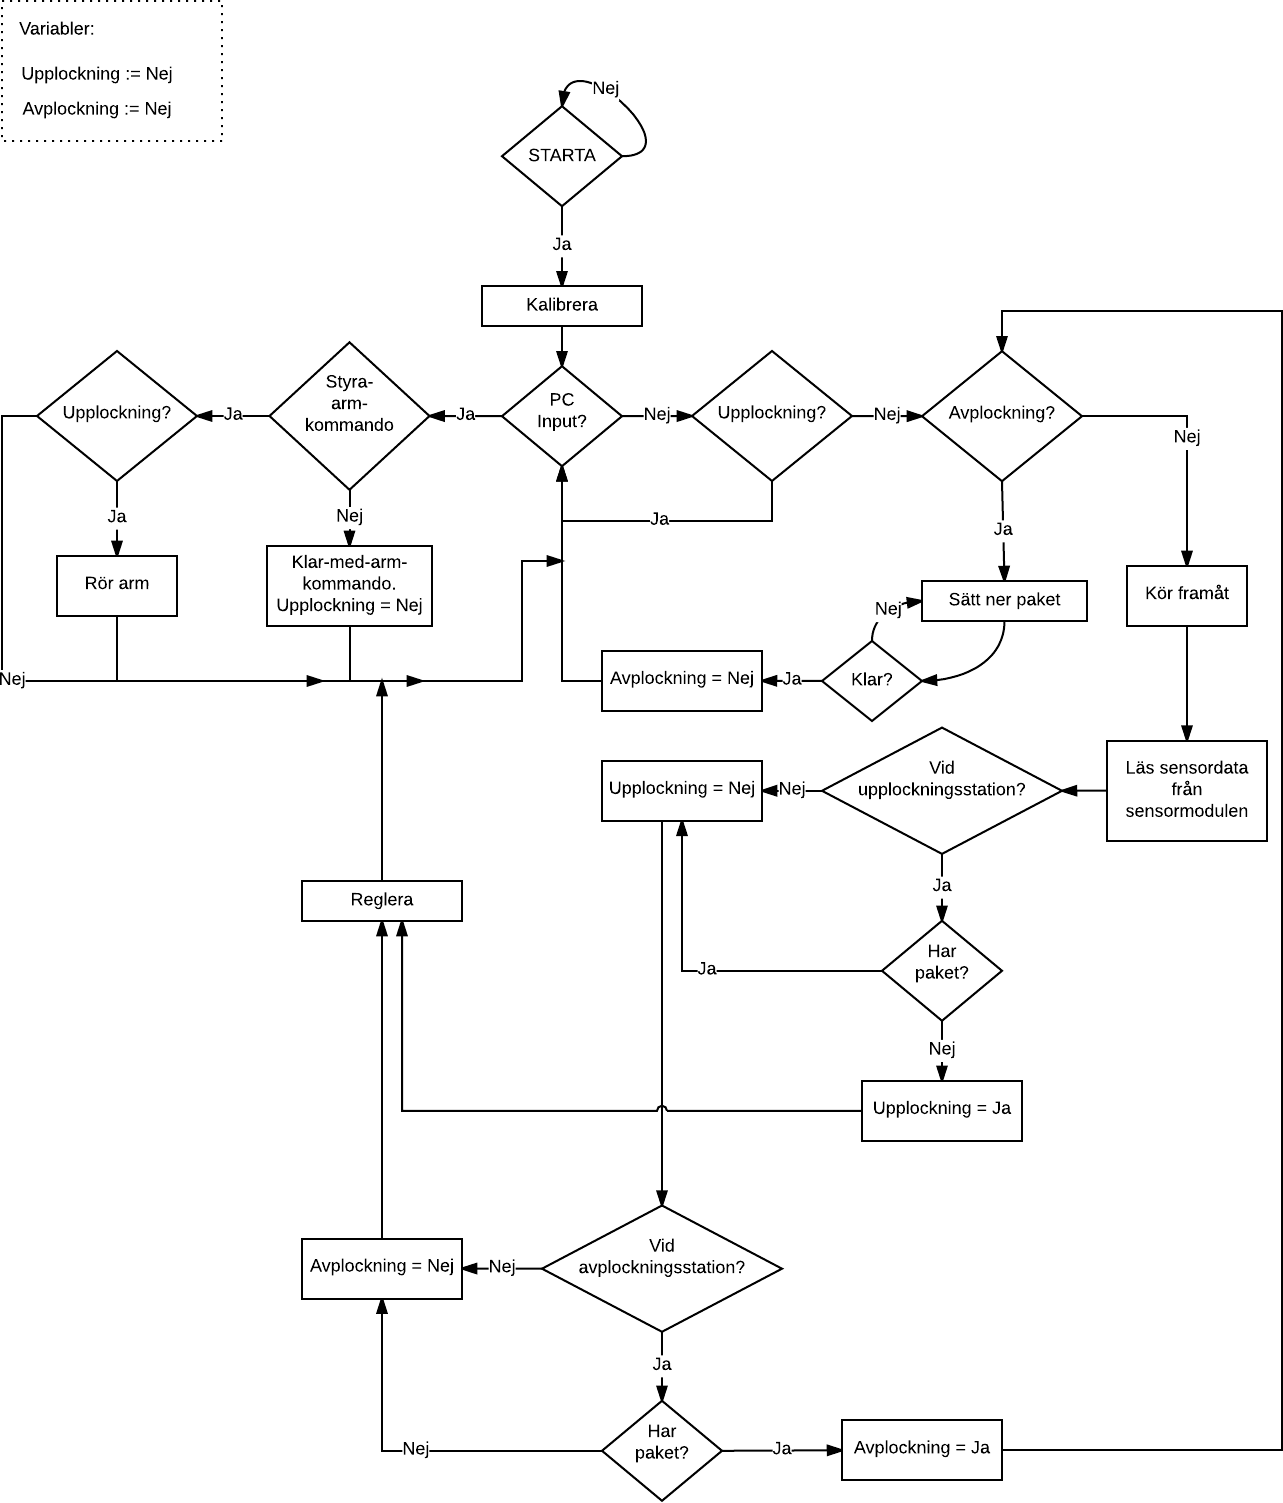
\includegraphics[scale=0.2]{grafik/huvud-styrlogik.png}
\caption{Flödesschema för huvudmodulens styralgoritm.} \label{systemskiss:autonomtschema}
\end{figure}

Figur \ref{systemskiss:autonomtschema} är en visualisering av hur det autonoma läget kommer att styras. Med hjälp av två stycken flaggor, Upplockning och Avplockning, kan systemet avgöra om den ska plocka upp eller lämna av ett paket eller bara fortsätta köra framåt längs banan. När Upplockning är satt till "Ja" väntar systemet på att användaren ska styra armen och sedan skicka ett "färdigt-kommando".
\subsubsection{Arbetsblock}
\begin{itemize}
\item Vänta på startsignal
\item Kalibrera sensorer
\item Hämta sensorvärden från sensormodul
\item Beräkna nästa lämpliga operation
\item Skicka kommandon till styrmodulen hur roboten ska färdas
\item Reglera för att följa linjen
\item Om upplockning ska ske:
\newline
Vidarebefordra kommandon från användaren till styrmodulen för armen
\item Skicka sensorvärden till användaren
\end{itemize}

\subsection{Manuellt läge}
När roboten är satt i manuellt läge väntar huvudmodulen på kommandon från användaren och utför sedan dessa.
\subsubsection{Arbetsblock}
\begin{itemize}
\item Hämta kommandon från användaren
\item Vidarebefodra kommandon till rätt modul
\item Skicka sensorvärden till användaren
\end{itemize}


%\documentclass[a4paper,11pt]{article}
%\usepackage[a4paper]{}
%\usepackage[utf8]{inputenc}
%\usepackage{listings}
%\usepackage{graphicx}
%\begin{document}

\section{Sensormodulen}
Sensormodulen har som uppgift att läsa in data från robotens sensorer, omvandla dem om det är nödvändigt och vidarebefodra dem till huvudmodulen. För att roboten ska kunna hitta behöver den först veta vart den är och till detta så används två stycken linjesensorer. För att kunna detektera paket kommer roboten på var sin sida ha två avståndssensorer. Om det finns tid så ska det sitta en linjesensor på armen för att kunna detektera formen på paket vilket möjligör utökning till autonom upplockning.

\subsection{Reflexsensormodul}
För att kunna beräkna vilken vinkel roboten har i förhållandet till linjen som den följer så har den en reflexmodul fram och en bak. Dessa består av 11 stycken reflexdetektorer som består av en lysdiod och en ljuskänslig transistor. Varje detektor har en enable ingång som slår på ljusdioden och en OUT utgång som ger en analog signal mellan 0V och 5V. Dessa kommer läsas av var för sig och när en detektorer inte läses av kommer enable vara låg för att inte påverka närliggande detektorer samt för att de inte ska överhettas. Avläsningen kommer att ska med två muxar av typen MC14067B vilket är en analog mux med 16 kanaler.
\subsubsection{Arbetsblock}
\begin{itemize}
\item kalibrera värden
\item ställ in muxarna
\item vänta på lysdiod för att stabilisera sig
\item läs av analog värde
\item omvandla analog värde till digital
\item ta hänsyn till kalibreringen om det är en tejp eller ej under detektorn och trunkera datat efter detta
\item skicka värden till huvudmodulen
\end{itemize}
\subsection{Avståndssensor}
För att kunna detektera om det är ett paket på någon sida av roboten vid stationer så kommer det sitta en avståndssensor på vardera sida av roboten. Dessa kommer vara av typen GP2D120 som är en avståndssensor som använder IR för att generera en analog signal. Denna signal är ej linjär så antingen måste funktionen linjäriseras alternativt så används ett lookuptable som den interpolerar över. Då muxarna som används till reflexsensormodulen har 16 kanaler och de endast använder 11 så kopplas dessa in samma. Dessa kommer dock vara aktiverade hela tiden.
\subsubsection{Arbetsblock}
\begin{itemize}
\item ställ in muxarna
\item läs av analog värde
\item omvandla analog värde till digital
\item kolla upp avstånden i ett lookuptable
\item skicka värden till huvudmodulen
\end{itemize}
\subsection{Flödesschema}
\centerline{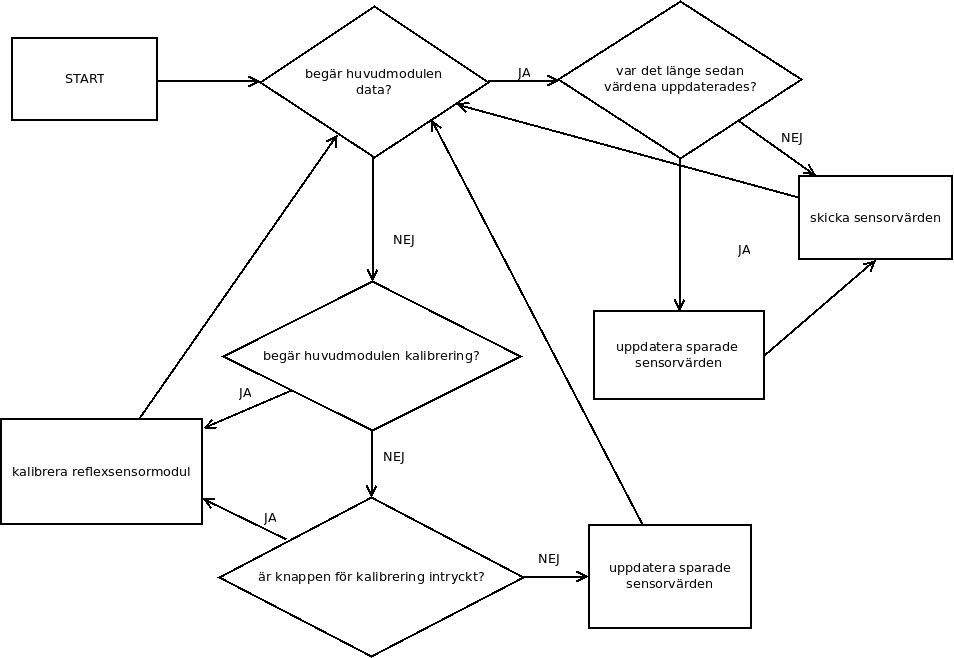
\includegraphics[scale=0.4]{sensorflow}}
\centerline{Flödesschema för sensormodulen}
%\end{document}


\section{Styrenhet}

Styrenheten har till uppgift att driva de motorer som driver hjulen och de servon som styr armen.Eftersom styrenheten kommunicerar med huvudmodulen genom UART kommer kommandon att tolkas med avbrott. Förslagsvis ska en Atmega16 microcontroller användas

\subsection{Framdrivning}

Motorenheten innehåller två hjulpar, de styrs separat för att göra det möjligt att svänga. Huvudmodulen skickar kommandon för hur snabbt vardera hjulpar skall rotera, styrenheten ser sedan till att motorerna kör i den efterfrågade hastigheten. Detta sker dock utan någon återkoppling från den verkliga hastigheten utan vi mäter upp vilken signal till motorerna som ger vilken hastighet och sedan används detta för att styra hastigheten under användning.

\subsubsection{Arbetsblock}
\begin{itemize}
\item Ta emot kommandon från huvudmodulen om vilken hastighet båda hjulparen ska hålla
\item Omvandla hastigheten till lämpliga PWM signaler
\item Starta motorn mjukt 
\item Lägg PWM signalerna på motorernas utgångar 
\item Stanna motorn mjukt
\end{itemize}

\subsection{Robotarm}

Robotarmen består av 7 servon av modell AX12-A. Dessa styrs genom att en målvinkel sätts (0-1023), med möjlighet att ändra hastighet, vridmoment och styra av/på. Från huvudmodulen får enheten målvinklar för varje enskild led. Styrmodulen är ansvarig för att se till att parallella servon körs synkroniserat, för att inte slita sönder varandra. Styrmodulen ansvarar också över att armen inte ska kollidera med resten av roboten. Den kommer att programmeras med vilka rymdmängder som den ej får passera och om den får kommandon som gör att den kommer passera dessa mängder måste den välja en annan väg än rakaste vägen.  
%\newline
%\centerline{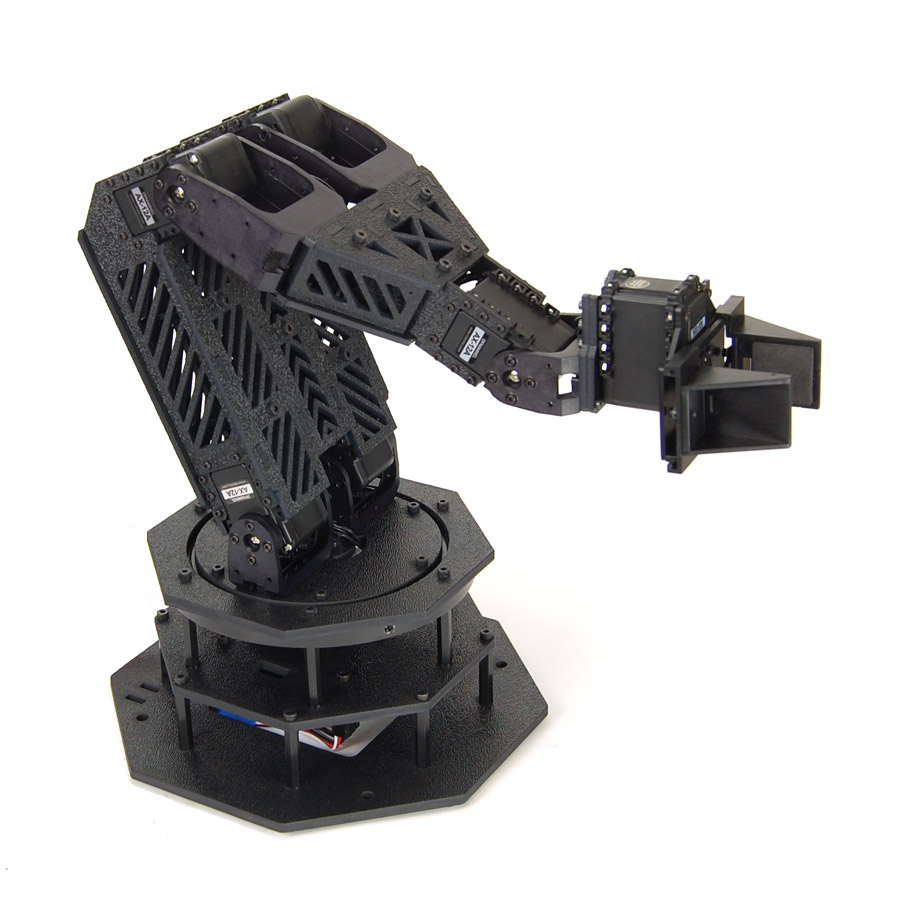
\includegraphics[scale=0.4]{arm}}

\begin{figure}[h]
\center
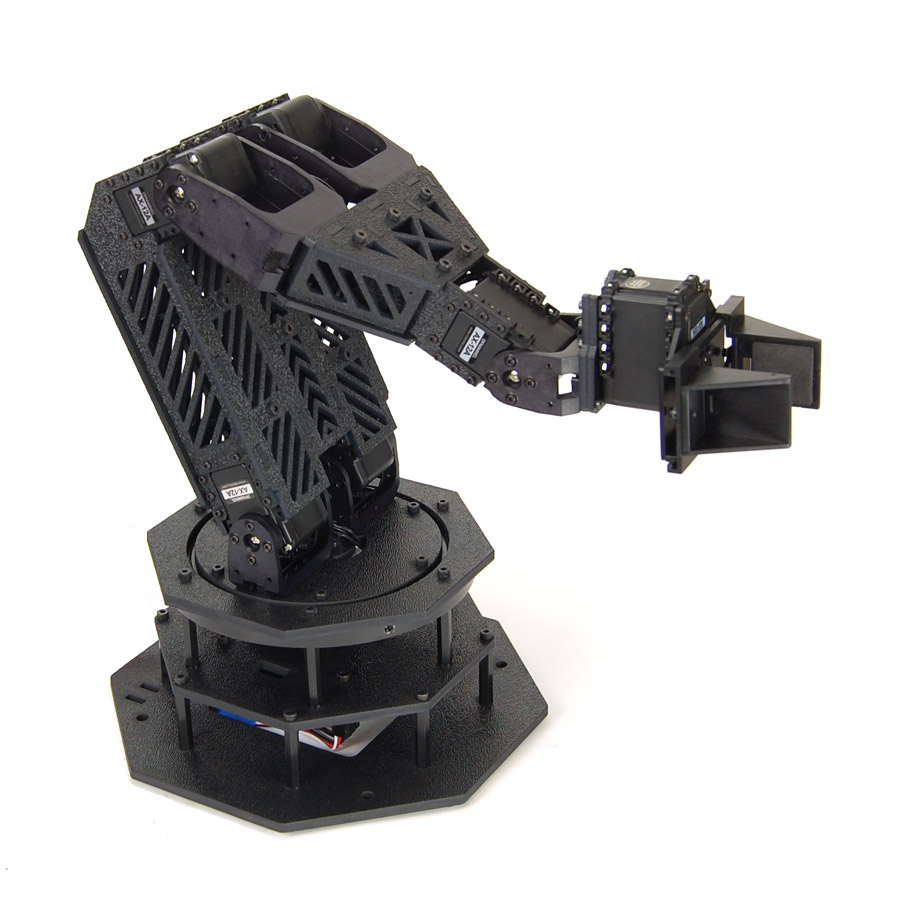
\includegraphics[scale=0.35]{arm}
\caption{Robotarm.}
\end{figure}

\subsubsection{Arbetsblock}

\begin{itemize}
\item Ta emot kommandon från huvudmodulen om vilka vinklar alla servon ska ha
\item Kolla om armen kommer röra sig igenom förbjuden rymd och beräkna en alternativ väg
\item Skicka kommandon till servona och se till så att de rör sig mjukt
\end{itemize}


\newpage
\begin{appendices}

% Bilagor

\end{appendices}


\end{document}
